% Planeringsrapporten ska tydligt ange ämnet/problemet som kandidatarbetet ska avhandla, samt hur detta ska göras. Följande rubriker och information ska vara med. Notera att följande rubriker skall vara med oavsett om studien är helt litteraturbaserad, innehåller en empirisk undersökning, eller är ett konstruktionsprojekt.

% Tidsplan
% Den här delen av planeringstrapporten beskriver vad som ska göras och när det ska göras. Personer som ska kontaktas bör också stå med här. Datum eller åtminstone veckor då studenterna ska ge delrapporter samt slutgiltiga presentationen ska stå här. Tidsplanen, kommer naturligtvis vara rätt grov i början.

% Det är viktigt att notera att aktiviteterna inom projektet inte kan ske sekventiellt då dessa aktiviteter är beroende av varandra, vilket innebär att ett antal iterationer mellan dem kommer att ske. Endast genom att iterera mellan dem kommer den uppbyggda kunskapen bli utnyttjad på ett bra sätt. Samma tänkande gäller också rapportskrivandet, d.v.s. uppdatering av ett avsnitt kräver att man uppdaterar andra. Rapportskrivande ska därför ske kontinuerligt under hela projektet.

\chapter{Time plan}

The purpose of this chapter is to arrive at a time plan out of the current perspective. It is possible to plan for execution of tasks but not whether it will be successful or not. As the project evolves, when new information and experience emerge, the plan will change and extend to include more tasks. 

A breakdown of the use cases for the AI resulted in the following list, sorted in the order of a probable development sequence:

%In planning the project, there are requirements set up that break up the project into smaller tasks. These can be executed both sequentially and in parallel. The requirements are a guideline for the project and gives concrete tasks that need to be completed before moving onto the next task. In this section these requirements are stated, given an execution order as well as a deadline. These may be subject to change as the projects moves along.
%\section{Requirements}
%The requirements in this project applies to different parts in the project and implementation. These requirements are set to make sure that there is an application with an AI that can execute some of the tasks given, and that there is a proper presentation and debug tool.
  
%\subsection{Specific AI requirements / AI behaviour development}

\begin{enumerate}
  \item Make the car drive on a straight.
  \item Be able to follow a curve.
  \item Be able to drive though a sequence of curves.
  \item Optimise time spent though a single curve by ...
    \begin{enumerate}
        \item ... adapting the speed.
        \item ... adapting the car's positioning.
    \end{enumerate}
  \item Optimise time spent though a sequence of curves by ...
    \begin{enumerate}
        \item ... adapting the speed.
        \item ... adapting the car's positioning.
    \end{enumerate}
\end{enumerate}

Again, it is difficult to prove that all the target behaviours will be met. But, the list, possibly in a edited form, will be used throughout project to set current complexity level. It is probably not realistic to pursue a latter goal before the previous ones has been accomplished. Keeping a limited scope for which the ai should be able to perform is probably useful for the problem solving process.


% TODO Martin. Kolla här! Bra sammanfattat, rätt förklarat?
Initially, an algorithm with the following components will be pursued:
\begin{enumerate} 
    \item Neural network as knowledge model
    \item Reinforcement learning with neuroevolution.
    \item Stochastic modification of edge weights
    \item Stochastic modification of topology
    \item Management of species
\end{enumerate}

In practice, the implementation will need to contain both the algorithm but also other parts to have a operational tool. The general algorithm parts are:

%\section{Method requirements / Machine learning architecture parts}

\begin{enumerate}
    \item Neural network
    \item Input from and output to simulation handling
    \item Retrieval of score from a simulation test
    \item Mutation of the network
    \begin{enumerate}
        \item Adjust weights
        \item Change topology
    \end{enumerate}
    \item Management of networks; species, generations and such.
\end{enumerate}

%\section{Other application requirements}
Other necessary parts of the application are:

\begin{enumerate}
  \item Representation of the track
  \item Visualisation of the track and car that is driving
  \item Simulator
  \item Ability to save and load knowledge models.
  \item Visualisation of knowledge models.
\end{enumerate}

\section{Schedule}
A plan has been determine for the initial tasks in the project, and is presented in the following pert chart. Details of the implementation, theoretical knowledge and decisions will be discussed and pursued throughout the project

\begin{figure}[!ht]
  \caption{Pert chart for the following weeks of the project.}
  \centering
    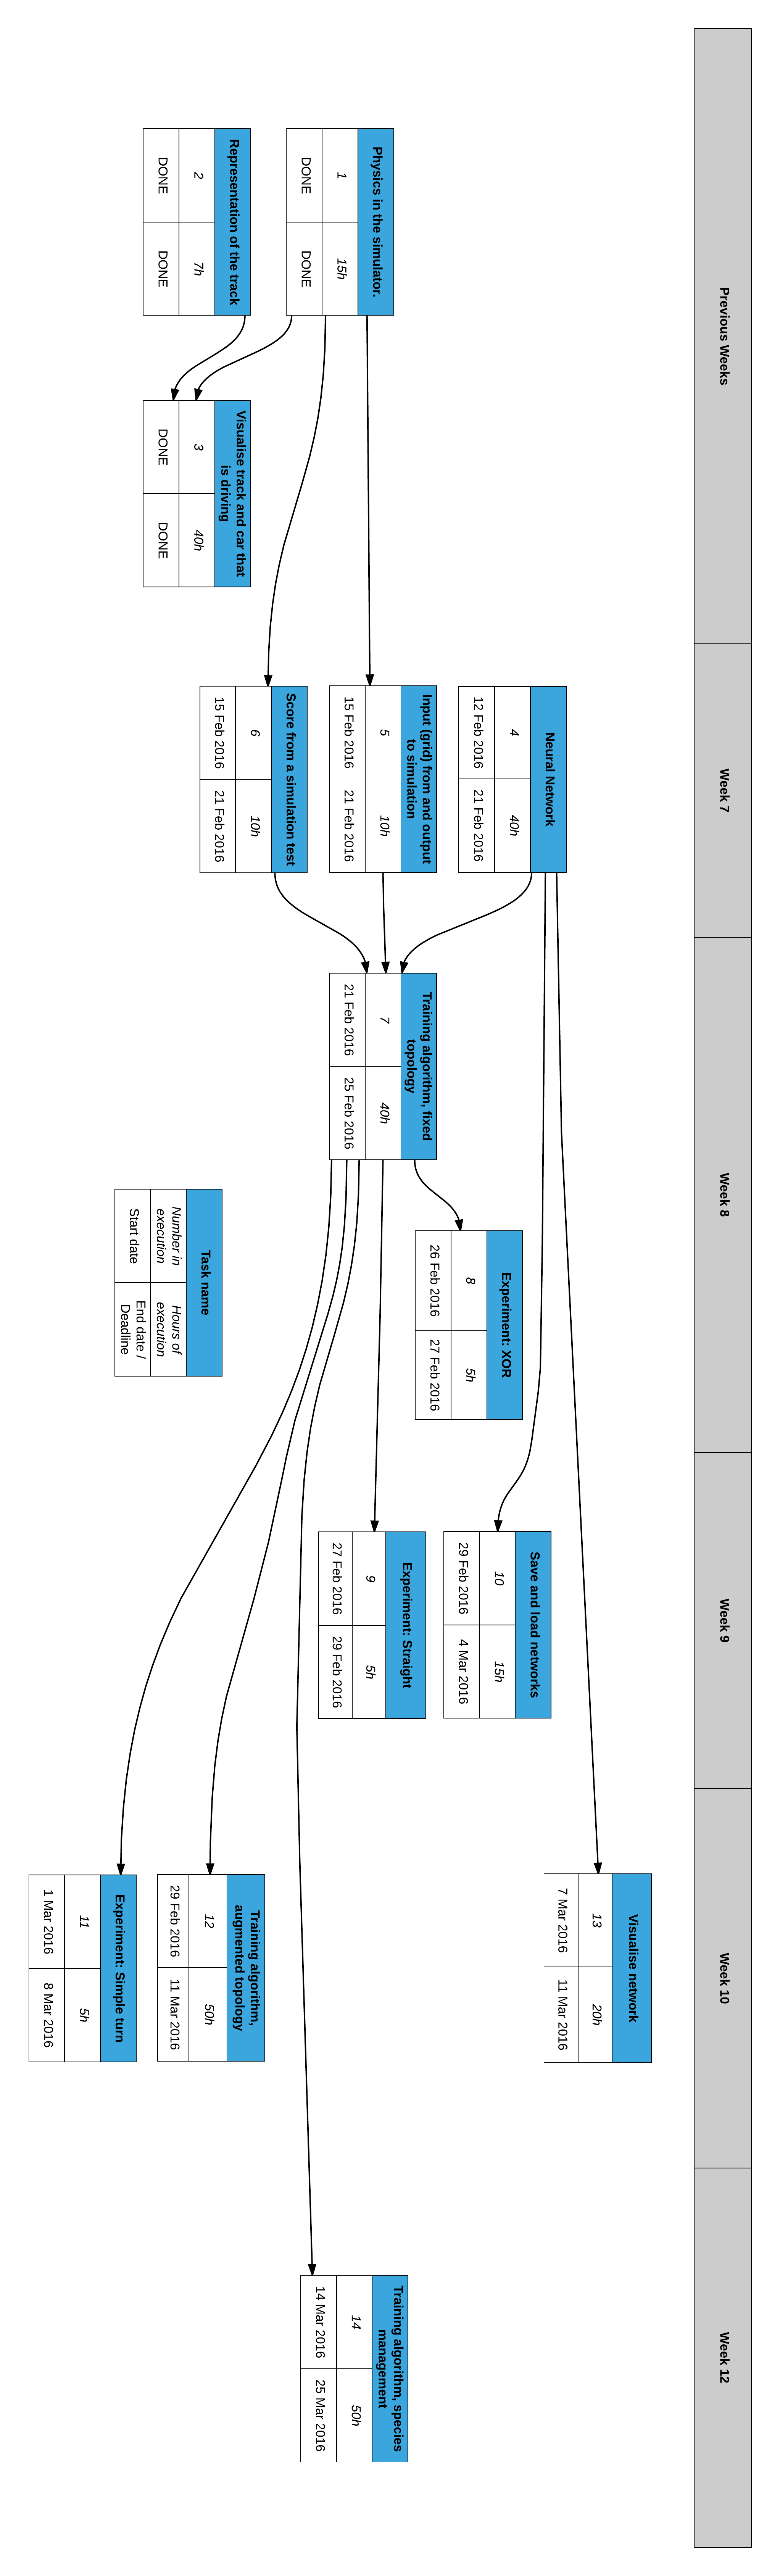
\includegraphics[scale=0.35]{PertChart}
\end{figure}

\iffalse
* What to do and when to do it.
* High resolution/detail a few weeks ahead, less details further ahead.
* Work in iterations and update the time-plan so that it stays relevant.
* Don't be too abstract.
* If we know what to do, don't plan too much, DO.
* If we are not sure about what to do, or how to do it - PLAN.
* IE. focus on planning the areas where we aren't certain of.


Simulation
Visualisation
    Car and Track
    Network
Basic program structure/architecture

Ai algorithm
    Neural network
        Nodes, edges, basic operations
        Save/load to/from file
    Connection to simulation, feedback.
    Simple training algorithm first
    ...
    MarI/O training algorithm - Evolving Neural Networks through Augmenting Topologies. 
    
\fi